
%\begin{abstract}
 
%\end{abstract}


%*****************************************
\chapter{Introduction}
%*****************************************

% introduction
%	- general topic
%	- motivation (why is it necessary)
%	- problem statement (major issues, problem parts, %		proposed solution)
%	- overview of thesis structure
	
% general topic, motivation
\section{Motivation}
With the ever increasing number of hard- and software systems that generate continuous streams of heterogeneous data it becomes more difficult to extract meaningful information from this data and act upon it in real time. 
Complex Event Processing (CEP) is a method that allows processing data streams from multiple sources by letting users specify events of interest as SQL-like queries and event patterns. These events are called complex events and result from the combination of several simple and other complex events through aggregation, composition and derivation operators.

If processing is performed centrally on one computing node, scaling of the system in terms of joining data sources, additional queries or an increase of the data rate is obviously limited. 
Therefore, distributing the operators involved in the processing of the data over several computing nodes is beneficial, if not necessary, in many application scenarios.

Since applications that have to react in real time to occurring events require a certain Quality of Service  (QoS) from the CEP engine, a solution to include QoS demands in a CEP system has been proposed with AdaptiveCEP \cite{Weisenburger2017a}. %TODO working reference to AdaptiveCEP paper
It allows the specification of QoS demands on queries, e.g. that the end-to-end latency from data source over all participating processing nodes to the user has to be less than 100ms, or that the frequency of received events has to be above a certain rate. 

To satisfy such requirements, the choice of a fitting placement algorithm is crucial; it is responsible for the distribution of individual processing steps of a query onto a network of processing nodes. Placement algorithms differ in the QoS metric(s) they optimize as well as the assumptions they make about the state of the network of processing nodes; these two aspects together constitute the context the system is operating in. Because of this, employing the wrong placement algorithm in a given context can have serious negative impact on the relevant QoS metrics and degrade performance of an application relying on the CEP system. 

\section{Problem Statement and Contribution}
While in a static context only the initial choice of the placement algorithm is important, in an application scenario with dynamic context the optimal placement algorithm may change over time because the network conditions or QoS demands can change significantly. Such a change is called a transition, from one context to another. The aspects that can be responsible for such a transition are, among others, node topology (clustered vs. distributed) and traffic type (burst vs. uniform). 

% adaptation here refers to changes the system makes because of periodic recalculations to adapt to slight changes in network conditions;
% reconfiguration refers to changes in the adaptation strategy and its mechanisms (== adaptation on a higher level)
%TODO check for consistency with weisenburger paper, section 4B
An adaptation strategy consists of several mechanisms (e.g. placement algorithm, query optimization) that determine how the system reacts to relatively small changes in the network QoS metrics.

The ability to dynamically reconfigure the adaptation strategy and its mechanisms at run-time based on the context is necessary to assure stable and reliable system operation in the face of significant changes in network conditions and user demands. 
In this work we will focus on reconfiguring the most influential mechanism, namely the deployed placement algorithm, but any other mechanism could be reconfigured as well. 

% problem statement (major issues, problem parts, proposed solution)

In order to perform reconfigurations of the adaptation strategy at run-time, we need two pieces of information: first, up-to-date information on the current context to determine if a significant transition has occurred and what the new context is; and second the most fitting mechanism(s) for the new context after the transition.
 
%Context information is, according to Etzion: \textit{" [...] indirectly relevant information that is useful to functioning of the service, but not provided to the service as part of its invocation"}, so in our case, any information that is relevant for determining what mechanism to use (i.e. information about network conditions, network QoS metrics, QoS demands), but is not provided by the user as part of a query. 
%TODO source (Etzion paper)
%TODO problem: qos demands are user-provided, but they are (very) relevant for determining what mechanism to use -> context or system in CFM? more logical to keep it together with query qos metrics

According to Dey \cite{}, context is \textit{"any information that can be used to characterize the situation of an entity. An entity is a person, place, or object that is considered relevant to the interaction between a user and an application, including the user and application"}. %TODO quote source (Dey Paper)
In our case, relevant information is any information that helps determining what mechanism to use (i.e. information about network conditions, network QoS metrics, QoS demands) without the user having to specify it.
This information must be captured in a structured way so that it can be automatically processed and used to determine the placement algorithm to be used. 
 
Due to the inherent variability of both system (utilized placement algorithm, processing nodes) and context we need a modeling technique that is suited to capture the possible configurations of our system and its context in a coherent way.
 
 Among the modeling techniques that can be used to construct a model representing the current state of system and context, we propose to make use of Feature Models (FM) to model system and context together in a Context Feature Model (CFM). %TODO sources

Feature Models have their origin in Software Product Lines (SPL) that represent different variants of a software system. They are used to specify variation points and the possible alternatives (features) at these points as well as constraints between these alternatives. A product configuration is created by 
 selecting or deselecting every feature, and is only valid if it respects all constraints between features.
 
 As the several variable parts of the context are important for deciding what adaptation to make in the system, modeling them as separated System Features (directly configurable system parts, e.g. placement algorithm) and Context Features (influences that cannot be controlled directly, e.g. network metrics, QoS demands) together in one model is a reasonable choice.
 By interpreting different context states as different configurations, we can identify transitions between contexts by observing changes in the configuration of the CFM. 
 
 % reference to Saller paper, where reconfiguration of the system is handled by a transition system; number of possible reconfigurations is limited through constraints between context features and system features, which allows
 By structuring the model through constraints and dependencies (between context features and system features as well as among context features) the space of possible configurations is limited to valid ones. This limits the amount of possible reconfigurations of the system, in our case the choice of the placement algorithm, to those allowed by the model.  
 Our aim is to determine the most fitting placement algorithm for a given configuration of Context Features; to achieve this, we propose to either predict the performance of every placement algorithm that is allowed by the constraints in this context configuration through some form of regression, or train a classifier to predict the most fitting placement algorithm based on the current context. 
 %TODO to keep or not to keep?
 In the first case, model constraints limit the number of different placement algorithms to be considered for a given context; in the second case, the amount of required training data is limited to instances with valid context configurations.
 
 Choosing a fitting placement algorithm would enable the system to adapt to known situations as well as new ones without the need for manual reconfiguration of the employed placement algorithm.


% thesis goals/aims

This thesis aims to explore context transitions in CEP systems and how to model them in order to enable self-adaptation of the system's adaptation strategy, specifically the placement algorithm. 
For this, we will first be reviewing relevant literature on context modeling, especially with the help of feature models, and context-based adaptation. Then we will identify required properties of a Context Feature Model to represent an adaptive CEP system, and design a model based on our findings. Next, a machine learning approach for placement algorithm selection will be chosen. 

To prove the applicability of our approach, the existing CEP system AdaptiveCEP will be extended with a prototypical implementation of the designed context model and a module that allows adapting the deployed placement algorithm at run-time based on the context information gathered by our model. The implementation will be evaluated for selected application scenarios to determine if it is able to improve system performance as intended.


% structure overview
%TODO adapt as necessary
\section{Outline}
The remainder of this document is structured as follows: 
chapter 2 includes background information on the topics of Complex Event Processing, Context Feature Models and Machine Learning and surveys and analyzes related work in the area of Context Feature Models in Dynamic Software Product Lines and adaptive CEP systems. Furthermore we will introduce an application scenario to give a practical example to refer to in the next chapters.
 In chapter 3 we will perform a context model requirement analysis for AdaptiveCEP, present and justify our CFM design and explain the prototypical implementation of the model and the adaptation mechanism.
 Chapter 4 covers the evaluation methods, results and their discussion
 In the final chapter 5 we will recap the thesis and reflect on the proposed solution and its results as well as possible future work.



\chapter{Background}
% general introduction into topics relevant to the thesis

%This chapter should give a comprehensive overview on the background necessary to understand the thesis. The chapter should have a length of about five pages!

\section{Complex Event Processing}

\subsection{Basics}
%TODO adapt, taken from old intro

Data sources (producers) generate streams of data in the form of simple events (e.g. sensor readings) which can be aggregated and combined with other simple or complex events and domain knowledge to create complex events. 
Interested parties (consumers) can define queries on event streams as complex events that can represent situations (specific event patterns) or specify further processing (aggregation, composition) of events.
If event patterns matching the query are detected in the event stream, the CEP engine will notify any interested consumers immediately.
This allows for timely reaction to new information by the consumers, making a whole range of new monitoring applications possible.

%TODO re-use and re-write partly if possible
%==== from OLD QOS+placement introduction, related work(placement) ====
This becomes even more important if the producers and consumers are constrained by certain QoS demands, e.g. in a scenario with geographically spread out producers and consumers where a certain end-to-end latency must not be exceeded. In this case it is not possible to route all events to a central processing node as it will likely cause the latency limit to be exceeded. Therefore the computations involved in processing a query need to be distributed across several nodes.

To find and maintain a mapping of the query (in the form of a logical flow graph consisting of sources, operators and drains) to the network hosts that satisfies all QoS demands imposed on the query, placement strategies are utilized. 
These strategies primarily handle the placement of the individual operators on hosts and try to optimize one or more QoS metrics in doing so and are periodically re-evaluated to check if the placement is still optimal or needs to be adjusted. 
These QoS metrics can be, among others: 
\begin{itemize}
\item latency 
\item bandwidth utilization
\item load balance
\item cost of transport and processing
\item reliability
\item availability
\item energy consumption
\end{itemize}

Currently, most operator placement algorithms used in practice focus on optimizing latency and/or load balancing. 
The placement of the operators cannot happen in an arbitrary way: some operators require a minimum of processing power or specific hardware; this is further constrained by sequential dependencies between operators: if an operator combines several simple or complex events, the operators that process these events need to be placed on processing nodes located upstream (viewed from the drain) of this operator's processing node, so this can reduce the number of feasible solutions. 

Further mechanisms to satisfy QoS demands involve the optimization of the operator graph as well as parallelization by replication of operators.

The choice of the appropriate strategy and its mechanisms depends on both the network conditions and the QoS demands imposed on the queries by users. As both can change over time, some form of context awareness and adaptability is necessary to guarantee a steady level of system performance.


As some applications have specific requirements regarding the network conditions to function as intended, AdaptiveCEP offers the possibility to include QoS demands with every query. These QoS demands, e.g. end-to-end latency < x or bandwidth > y, are used to ensure that every host between source and drain involved in the processing of a query helps satisfying these requirements. 

\subsection{Quality of Service in CEP}
\subsection{Adaptation mechanisms in CEP}
%placement algorithms

To find and maintain a mapping of the query (in the form of a logical flow graph consisting of sources, operators and drains) to the network hosts that satisfies all QoS demands imposed on the query, placement mechanisms are utilized. 
These mechanisms primarily handle the placement of the individual operators on hosts and are designed  for specific situations characterised by network conditions like traffic type (bursty or uniform), network topology (distributed or clustered), stability of connections and queries, and to optimize one or more QoS metrics. This makes the choice of the most fitting placement mechanism crucial for the system performance. 

Most mechanisms periodically re-evaluate to check if the placement is still optimal or needs to be adjusted. While periodic re-evaluation of the placement enables the system to react to changes in the underlying network to a certain degree, there is currently no way to adapt the utilized placement mechanism to major changes of the application context that affect the QoS demands in an automated way.
If any part of the application context (e.g. network conditions, network topology, consumers' preferences of QoS metrics) is changed significantly, the placement algorithm that was used before may no longer be optimal as it was intended for a different context.

%TODO include relevant parts
The paper Placement Strategies for Internet-Scale Data Stream Systems  by Geetika T. Lakshmanan, Ying Li and Rob Strom is a survey of 8 algorithms developed to solve the problem of optimal operator placement in data stream processing systems. To compare the different approaches, the authors define a set of core components that significantly affect the performance of the system and compare the categories of these components: 

\begin{itemize}
\item architecture (centralized, decentralized or hybrid implementation of placement logic)
\item algorithm structure (centralized vs decentralized decisions)
\item metric(s) to optimize (load, latency, bandwidth, machine resources, operator importance, combinations of those)
\item operator-level operations (reuse or replication of operators) 
\item reconfiguration (triggers for operator migration: thresholds, periodic re-evaluation, constraint violation)
\end{itemize}

Based on these components, 8 placement algorithms developed respectively by Pietzuch, Balazinska, Abadi, Zhou, Kumar, Ahmad, Amini and Pandit are assigned to the discussed categories. The authors then proceed by comparing the algorithms w.r.t. their design decisions and underlying assumptions. It is concluded that decentralized approaches which are able to adapt dynamically by operator migration are prevalent, with latency and, by extension, load balancing being the preferred metrics to optimize. 
Based on the comparison of the assumptions a decision tree for selecting a fitting placement algorithm considering the characteristics of a given problem (node distribution, number of administrative domains, dynamics of topology and data, query diversity) is proposed.


%=====================================================

\section{Context-Awareness and Adaptive Systems}

\section{Context Modeling}
\subsection{Types of Context Models}
\subsection{Dynamic Software Product Lines and Feature Models}
\subsection{Context Feature Models}

\section{Machine Learning}
\subsection{Regression Learning}
\subsection{Classification}

\section{Summary}


\chapter{Related Work}
% relevant work on related topics
% categorize, evaluate, summarize other works, show differences and parallels; similar solutions but not necessarily similar problems; understand limitations of other works -> avoid them if possible)

%This chapter should give a comprehensive overview on the related work done by other authors followed by an analysis why the existing related work is not capable of solving the problem described in the introduction. The chapter should have a length of about three to five pages!
\section{Context Modeling for Event-based Systems}

\subsection{Context Modeling Techniques}

%move this information to background?
Freudenreich explicitly differentiates between situation context (information about environment) and interpretation context (information about data). Regarding the modelling of situational context of event-based systems he identifies the following required features and characteristics, based on three surveys of different context models: 
\begin{itemize}
\item aspects:
\begin{itemize}
\item absolute and relative space and time 
\item application as subject
\item no context history or user profiles
\end{itemize}
\item representation: 
\begin{itemize}
\item key-value based
\item low formality
\item fully general, variable granularity
\item no valid context constraints
\end{itemize}
\item management: 
\begin{itemize}
\item context construction distributed and at runtime
\item basic context reasoning
\item hooks for incompleteness and context information quality monitoring
\item multi-context modeling
\end{itemize}
\end{itemize}
After identifying these requirements, he argues that there is a need for relationship representation and basic reasoning, but ontology-based models, which provide elaborate context reasoning, are considered to be too detrimental to EBS performance. Therefore he proposes an ontology-based metamodel that can represent domain concepts in terms of concepts, attributes and relationships which allows for context construction to happen at runtime, while the context information structure is determined at design time. The metamodel makes no assumptions about the domain model's data types or structure, making it very flexible. Situations and reactions to them can be specified declaratively as policies using the defined ontology.

E.Barrenchea et al. propose to embed context information directly into events as a first class element. Components can specify the context of their publications and/or subscriptions. Components can be grouped into contextual environments ( making them "siblings") that share the same context parameters and values. Context awareness is realized by context filters in an environment middleware layer that filter according to the specified event schema and the environment they are part of, which relieves components of keeping track of context information directly. This moves context away from the component logic and towards the layer of the pub/sub scheme.  An environment manager handles context updates and provides an interface to the application layer for utilizing  context information.

Koripip\"a\"a et al. present a software framework for context acquisition and processing in mobile scenarios. The API uses an extensible context ontology to define usable contexts. The context schema is defined in RDF syntax to ease the sharing of the ontology. Context has six possible properties: (first two are mandatory) 1. type 2. value 3. confidence 4. source 5. timestamp 6. attributes. It is possible to create context hierarchies and composite contexts.
The framework consists of a context manager (blackboard, delivers context information based on subscriptions), a resource server (collects and preprocesses context data from sources) and context recognition services (create higher-level contexts from atoms, can be plugged in at runtime). The recognition services make use of Naive Bayes classifiers and the confidence property to create higher-level contexts.

\subsection{Feature Models for Context-Aware Systems}
Some authors propose using feature models, which have their origins in the domain of highly configurable software product lines (SPL), as a means to model the variability and behaviour of context-aware systems.

M.Archer et al. suggest using two separate feature models: one for the system and its variable parts, and one for the context, each of them with its own constraints (e.g. require, exclude). This allows for a homogeneous representation of system and context and the relationships between the two. The two models are then linked together by dependency constraints which represent the adaptation behaviour. The adaptation of the system happens based on event-condition-action (ECA) rules, with elements of the context feature model as condition and a re-configuration of the system feature model as the action part. The authors mention optimization of a utility function as an alternative to ECA-rules for modeling adaptive behaviour, which would require the feature model to be extended with attributes for information needed for the optimization.

Saller et al. aim to enrich feature models with context information and context constraints in order to limit the set of valid configurations further. This is done to limit the complexity of re-configuration planning and enable such calculations on resource-constrained devices. Reconfiguration is modeled and pre-planned in the form of a transition system, with transitions from one valid system configuration into the next, based on context. To further reduce the amount of possible transitions, states with different configurations that satisfy the same constraints are considered to be identical in terms of transitions (incomplete state space). This model allows for multiple contexts to be active at once.

Weckesser et al. propose an approach that extends the expressiveness of feature models as well as the possibilities to validate them. It allows for modeling  of feature attribute types and constraints beyond boolean as well as UML-like multiplicities of features. Furthermore, they enable automated validation of such cardinality-based feature models through methods that check the constraints imposed on the feature model by cardinality annotations. This is useful when dealing with systems that have multiple instances of a feature and need to take dependencies among them (and their number) and other features into account.

\section{Adaptation and Context-Awareness for CEP and other Event-based Systems}
% AdaptiveCEP paper

\section{Performance Prediction using Feature Models}
%TODO keep or remove?
SPLConqueror is a collection of programs and a library for discovering the influence of configuration options of software with variable elements on non-functional properties. This is done iteratively by using linear regression learning and stepwise feature selection. It consists of four programs: 
\begin{itemize}
\item VariabilityModelGUI: creation and editing of variability models of the configurable system; allows for exclude/require constraints between elements
\item PerformancePredictionGUI: learning an influence model from a given variability model and a set of measurements (of configurations and their performance regarding one metric). Possible configuration options for sampling and linear regression algorithm are available. The result is a an influence model of terms of weighted influences on one specific performance metric in the following form: (w1*c1 + w2*c2 + ... w34*c3*c4) where w34*c3*c4 denotes the selection of both configuration options c3 and c4
\item SPLConquerorGUI: GUI for visualization and analysis of the learned model with options for filtering variables and adjustment of the model. Visualization of influences and detected dependencies
\item CommandLine: allows for specification and execution of experimental setups with different sampling and machine learning options
\end{itemize}
 Further submodules include MachineLearning (algorithm for learning performance-influence model; interface for SAT checking of configurations w.r.t variability model and optimization of configuration for a given non-functional property and objective function) and PyML (interface to scikitlearn (a python ML framework), different regression learning techniques).
 
 Application to AdaptiveCEP: 
 1. determine from measurements for every mechanism (context (network conditions) -> performance (w.r.t. mechanism's optimized QoS metric?)) the influence of every context element on the performance metric by using linear regression; -> need to restrict combinations of context features + mechanisms to valid ones to limit necessary training/measurement data 
 2. the resulting formula (with weights for the influence of each context feature) can predict the performance of every context feature configuration for each mechanism 
 3. with this, calculate the predicted performance of every mechanism for a given context configuration
 4. compare the performance predictions of the different mechanisms for a given context configuration; problem: how to compare performance measured in different metrics? Can it be reasonably normalized to [0,1], if yes, what lower/upper bounds to choose for latency, bandwidth, ... to make them comparable?
 5. if reasonable comparison of performance metrics can be found: choose mechanism with best (normalised) performance for the given context

\section{Summary}

%Design
%This chapter should describe the design of the own approach on a conceptional level without mentioning the implementation details. The section should have a length of about five pages
% 1. Requirements + Assumptions 2.System Overview 2.1 Component A, 2.2 ..., 3. Summary

%This chapter should describe the design of the own approach on a conceptional level without mentioning the implementation details. The section should have a length of about five pages.

\chapter{Design of Context Feature Model and Mechanism Reconfiguration Approach}
% in detail: problem analysis, identification of important issues, describe and explain proposed solution, identify remaining issues

%TODO old motivation, re-use?
%If an application has to be capable of adapting to changing conditions in its execution environment, it needs information on the aspects that can change over time and are relevant for adapting its behavior. This is achieved by representing the context of an application in a context model. According to Dey, context is \textit{"any information that can be used to characterize the situation of an entity. An entity is a person, place, or object that is considered relevant to the interaction between a user and an application, including the user and application"}. Other definitions of context exist, such as the following by Etzion: \textit{"Context is indirectly relevant information that is useful to functioning of the service, but not provided to the service as part of its invocation"}. Both definitions imply that context information has to be collected and stored in a way that enables the application to ensure it behaves according to expectations. As every application has different notions of what context information is to be considered relevant, the required features of a context model need to be identified based on the desired behavior of the application.


\section{Context Feature Model Design}
\subsection{Application Requirements}
In the case of AdaptiveCEP, the system should be able to detect the conditions of the network that hosts the operators of its queries. In order to ensure the compliance with any QoS demands placed on the queries, it should then be able to dynamically choose appropriate mechanisms (operator placement strategy, ...) that fulfill the demands and optimize their relevant QoS metrics even if the network conditions change. 
To do this, the application needs knowledge about the status of any nodes currently hosting operators (to detect performance deterioration) as well as alternative nodes currently unoccupied (for possible reconfiguration).
Some of this information could be abstracted into coarser categories to facilitate decision making.
Furthermore, it should be able to cope with joining and leaving hosts. 
The adaptability of the application is given by the different strategies therefore it should be possible to include new strategies, possibly with new types of QoS metrics. Useful dimensions of network status information are, among others: latency, bandwidth, utilization, throughput, location/velocity (in case of mobile network entities), energy consumption.

\subsection{Context Model Requirements}
To capture the requirements of the context model in a structured manner, the analysis framework proposed by Bolchini et al. is used. This categorizes the requirements as follows: \\
1. Modeled Aspects \\
\newline
\begin{tabularx}{\textwidth}{|X|X|}
\hline
\textbf{Feature} & \textbf{Analysis Result} \\
\hline 
space & yes, necessary for proximity demands \\ 
\hline 
time & maybe, for "freshness" of information \\ 
\hline 
absolute/relative space and time (coordinates/timestamp vs. near/after something)  & abs.+relative space, absolute time \\ 
\hline 
context history (does the current context state depend on previous ones)  & unclear, maybe for stability metrics of links; needed for machine learning purposes? \\ 
\hline 
subject (what is the point of view -> user or app perspective) & app centric, system needs context information to optimize strategy usage \\ 
\hline 
user profiles (are user preferences relevant for the context, how are they represented) & Qos demands can be viewed as user preferences \\ 
\hline 
\end{tabularx} 


2. Representation Features \\
\newline
\begin{tabularx}{\textwidth}{|X|X|}
\hline
\textbf{Feature} & \textbf{Analysis Result} \\
\hline 
type of formalism (key-value, markup, logic, graph, ontology -> different intuitiveness, reasoning possibilities)  & Context Feature Model == graph-based, logic for constraints \\ 
\hline 
flexibility (domain specific vs general)  & specific to application, with enough flexibility for extensions \\ 
\hline 
variable context granularity (ability to represent context at different levels of detail) & - \\ 
\hline 
valid context constraints (can the number of possible contexts be restricted by semantic constraints) & necessary to restrict space of system configurations; inherent to CFM \\ 
\hline 
\end{tabularx} 
 
 3. Context Management and Usage \\
\newline
\begin{tabularx}{\textwidth}{|X|X|}
\hline
\textbf{Feature} & \textbf{Analysis Result} \\
\hline 
context construction (central description of possible contexts at design time vs distributed construction of the current context at runtime) &  central description of context dimensions, distributed construction by collection of current values \\ 
\hline 
context reasoning (ability to infer properties or construct higher-order context information from sensor readings) & maybe, abstract from measurements to situations \\ 
\hline 
multi-context modeling (one instance of the model can represent all possible context, not one instance for each context) & yes, need to model changes between contexts \\ 
\hline 
\end{tabularx} 

\subsection{Context Feature Model Proposal}
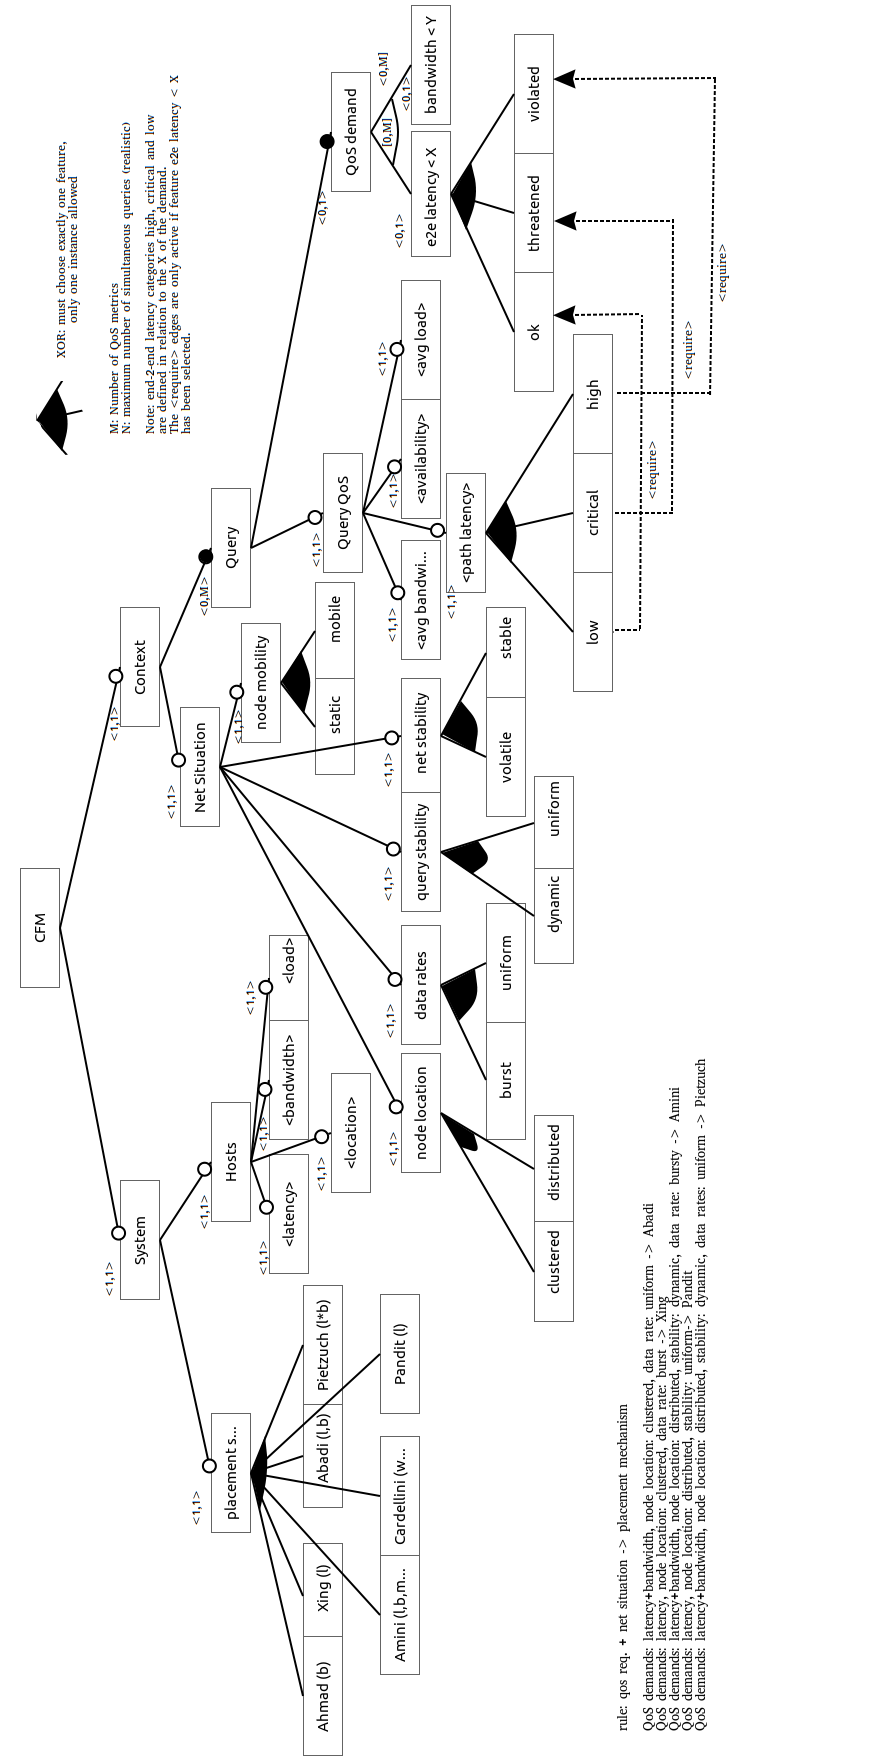
\includegraphics[scale=0.4]{alternative3.png}

Note: will split graph in system and context part for better readability 


The model limits itself to those elements of the system that are relevant for the detection of or reaction to network environment changes.
The graph modeling technique used to represent the context model as a feature model was first used in the domain of Software Product Lines (SPL) and allows definition of variable parts (features) of both system and context. At runtime, the active features constitute the configuration of the system/context; the space of possible configurations is restricted by constraints between features (xor-, or groups, require- and exclude relations). This allows the restriction of the model to valid configurations, which is helpful when gathering measurement data for different possible configurations. 
The main elements of the context are the queries executed by the system, their QoS metrics, the QoS demands placed upon them, and a set of situations that characterize the network conditions of the nodes in the system. These situations abstract from measurements on single hosts to the overall state of the queries' environment, and can be used in the definition of constraints and adaptation rules. Their mutually exclusive subcategories (like dynamic, uniform) can be defined by threshold values (in some relation to QoS demands on operators) and can be defined more finely granular if necessary. Note that multiple Situations can be active at the same time.
The variable parts of the System are the ones that can be directly reconfigured: the placement mechanisms, each optimizing a set of QoS metrics and suited to a certain situation. Although they can not be directly reconfigured, the Hosts/Nodes are an integral part of the system, so they are included on this side of the model. Every Host in the System has a set of associated QoS measurements.
For the sake of readability, constraints among the features of the model can as well be noted separately as follows: 
\newline
\begin{center}
 (C1) Situation:data rate:burst \textbf{and} Situation:node location:clustered \textbf{and} Query:QoS demand: e2e latency < X \textbf{requires} placement:Xing\\
 
 \end{center} 
with Xing being a placement strategy that aims to minimize the latency.
Adaptations from one strategy to another could be triggered in a similar manner:

\begin{center}
(A1) Query:QoS demand:latency \textbf{and} Query QoS:path latency:high \textbf{implies} other latency optimizing strategy\\

\end{center}

\section{Mechanism Reconfiguration Approach}
\section{Summary}

% Implementation
%This chapter should describe the details of the implementation addressing the following questions:
%1. What are the design decisions made?
%2. What is the environment the approach is developed in?
%3. How are components mapped to classes of the source code?
%4. How do the components interact with each other?
%5. What are limitations of the implementation?
%The section should have a length of about five pages.

% 1. Design Decsisions 2. Architecture 3. Interaction of Components 4. Summary
\chapter{Implementation}

Preliminary Implementation Considerations:
\begin{itemize}
\item context information could be distributed via context events; a context manager subscribes to context sources and the application (or adaptation strategy) subscribes to the aggregated events from the context manager
\item context source monitoring could happen similar to the existing MonitorFactories
\item create a new interface for the context elements (metrics, attributes, constraints) and its management
\end{itemize}


\section{Design Decisions}
\section{Architecture}
\subsection{Context Feature Model}
\subsection{Mechanism Reconfiguration Approach}

\section{Interaction of Components}
\section{Summary}


%This chapter should describe how the evaluation of the implemented mechanism was done.
%1. Which evaluation method is used and why? Simulations, prototype?
%2. What is the goal of the evaluation? Comparison? Proof of concept?
%3. Wich metrics are used for characterizing the performance, costs, fairness, and efficiency of the system?
%4. What are the parameter settings used in the evaluation and why? If possible always justify why a certain threshold has been chose for a particular parameter.
%5. What is the outcome of the evaluation?
%The section should have a length of about five to ten pages
% 1. goal and methodology 2. setup 3. resutls 4. analysis
\chapter{Evaluation}
\section{Methodology}
% describe how performance is measured

\section{Evaluation Setup}
% describe testenvironment setup
% describe test cases for transitions between contexts

\section{Results}
% compare system performance in test cases with and without context awareness (if there are implementation variants, compare these as well)
\section{Analysis and Discussion}
% does the solution improve performance, what issues are there and why


%This chapter should summarize the thesis and describe the main contributions of the thesis.
%Subsequently, it should describe possible future work in the context of the thesis. What are limitations of the developed solutions? Which things can be improved? The section should have a length of about three pages.
%1. Summary 2. Contributions 3. Future Work 4. Final Remarks
\chapter{Conclusion}
% brief recap of work so far, discuss findings of analysis -> what are strengths and shortcomings of the solution, new problems -> future work

\section{Summary}
\section{Contributions}
\section{Future Work and Final Remarks}


%*****************************************
%*****************************************
%*****************************************
%*****************************************
%*****************************************